\chapter{Специальная часть}
\section{Постановка задачи}
Разработать метод мониторинга состояния ЛА на основе методов интеллектуального анализа данных. Реализовать программную систему, использующую данный метод.

Система должна удовлетворять следующим требованиям:
\begin{itemize}
	\item строить модель системы только на основе телеметрии при различных режимах её работы, без априорных данных о её назначении, составе, конструкции (обучение без учителя);
	\item обладать способностью классифицировать аномалии в работе системы;
	\item обрабатывать большие массивы входных данных (несколько десятков тысяч точек) за конечное время;
	\item определять состояние системы в режиме реального времени.
\end{itemize}

\section{Анализ существующих методов выявления аномалий без учителя}
На данный момент существует несколько методов, для которых доказана возможность применения их в системах контроля и диагностики ЛА. Такими методами являются Orca, GritBot, IMS (Inductive Monitoring System), GMM (Gaussian Mixture Model), DBN (Dynamic Bayesian Network) и One-Class SVM (Support Vector Machine)~\cite{MartinCompUnsupervisedDetectionMethods}.

\subsection{Orca}
Orca~---~метод поиска аномалий без учителя, использующий подход «ближайшего соседа» (nearest neighbor) для поиска аномалий~\cite{SchwabacherMachLearnAppl}. Данный метод был разработан Стефеном Бэйем (Institute for the Study of Learning and Expertise) и Марком Швабахером (NASA Ames Research Center) и подробно описан в~\cite{BaySchwabacherOrca}. Orca относится к методам обнаружения аномалий, основанных на измерении расстояний между точками (distance-based).

Понятие аномалии для данного класса методов определено следующим образом: «объект $O$ в выборке $T$ является аномалией, если по крайней мере доля $p$ из всех объектов в $T$ лежит дальше от $O$, чем расстояние $D$»~\cite{KnorrNgDistBasedAlgorithms}. Distance-based методы являются обобщением некоторых статистических тестов на аномальность. Данный класс методов не требует априорных знаний о виде распределения для выборки. Кнорр и Нг предложили простейший алгоритм на вложенных циклах (Nested Loop, NL)~\cite{KnorrNgDistBasedAlgorithms}, который находит аномалии путём вычисления расстояния между всеми точками в исходной выборке. Сложность данного алгоритма составляет $O(kN^2)$, где $k$ --- размерность пространства, а $N$ --- размер выборки.

Несмотря на то, что были разработаны более эффективные c т.з. вычислительной сложности алгоритмы (\cite{TaoMiningDistBasedOutliersFromLargeDB}~и~\cite{AngiulliVeryEfficientMiningDistBasedOutliers}), на практике наиболее сложным является определение расстояния $D$, по достижению которого точку следует считать аномалией. Может потребоваться непредсказуемо большое число итераций, чтобы найти подходящее значение $D$. Найти интервал $[D_{min}, D_{max}]$ возможно путём полного перебора, как показано в~\cite{TaoMiningDistBasedOutliersFromLargeDB}, но данный подход обладает слишком высокой вычислительной сложностью.

В качестве решения данной проблемы было предложено следующее определение аномалии, не требующее задания $D$: «объект считается аномалией, если это один из $n$ объектов с наибольшим расстоянием до их $k$-ых ближайших соседей, где~$k,n\in\mathbb{N}$»~\cite{RamaswamyEffAlgoMiningOutliers}. Пользователю достаточно указать количество аномалий, которое должен вернуть алгоритм, без прямого указания дистанции $D$. Более того, возвращаемые алгоритмом аномалии будут ранжированы по степени аномальности, являющейся численной характеристикой.

Orca использует данный подход, развивая идею алгоритма на вложенных циклах~(NL). Данный алгоритм на больших массивах данных показывает сложность, близкую к линейной~\cite{BaySchwabacherOrca}.

Псевдокод алгоритма приведён в листинге~\ref{lst:spec:OrcaPseudocode}. Ключевыми особенностями алгоритма являются:
\begin{itemize}
	\item необходимость рандомизации исходных данных (строка~\ref{lst:spec:OrcaPseudocode:Random}). Для эффективной работы алгоритма требуется, чтобы объекты в выборке находились в случайном порядке. При обработке выборки на ПЗУ возможно рандомизировать выборку за линейное время и используя конечный объём памяти~\cite{BaySchwabacherOrca};
	\item использование вложенных циклов (строка~\ref{lst:spec:OrcaPseudocode:NL}). Основной идеей является отслеживание ближайших соседей для каждого объекта в $D$;
	\item правило отсечения (строка~\ref{lst:spec:OrcaPseudocode:Pruning}). Когда для ближайших соседей объекта степень аномальности становится меньше, чем величина среза, алгоритм удаляет данный объект, так как больше нет оснований считать его аномальным. Чем больше объектов перебирает алгоритм, тем выше становится величина среза, улучшая таким образом эффективность алгоритма по времени.
\end{itemize}

\begin{algorithm}[h]
\caption{Псевдокод алгоритма Orca}
\label{lst:spec:OrcaPseudocode}
\begin{algorithmic}[1]
\REQUIRE $k$, количество ближайших соседей; $n$, количество аномалий; $D$, выборка.
\ENSURE $O$, множество аномалий
\STATE Перемешать все объекты в выборке $D$. \label{lst:spec:OrcaPseudocode:Random}
\STATE Инициализировать величину среза нулём.
\WHILE{в выборке $D$ остались необработанные объекты}
	\STATE Загрузить фиксированное количество объектов $B$ в буфер.
	\FOR{каждого объекта $d$ в $D$} \label{lst:spec:OrcaPseudocode:NL}
		\FOR{каждого объекта $b$ в $B$}
			\STATE Вычислить расстояние между $b$ и $d$.
			\IF{$d$ ближе к $b$, чем $k$ ближайших соседей $b$}
				\STATE Заменить соседа с наибольшим расстоянием на $d$.
				\STATE Вычислить степень аномальности $b$.
				\IF{степень аномальности ниже величины среза} \label{lst:spec:OrcaPseudocode:Pruning}
					\STATE Удалить $b$ из $B$.
				\ENDIF
			\ENDIF
		\ENDFOR
	\ENDFOR
	\STATE Поместить в $O$ оставшиеся в $B$ объекты.
	\STATE Отсортировать объекты в $O$ по степени аномальности.
	\STATE Оставить в $O$ только $n$ объектов.
	\STATE Обновить величину среза степенью аномальности последнего объекта в $O$.
\ENDWHILE
\RETURN $O$.
\end{algorithmic}
\end{algorithm}

Преимуществами метода являются:
\begin{itemize}
	\item превосходная масштабируемость: на выборках большого объёма производительность алгоритма близка к линейной;
	\item низкие требования к памяти: не требуется загружать в память всю выборку;
	\item возможность задать любую метрику для расстояния и функцию для определения степени аномальности.
\end{itemize}

Недостатки следуют из природы метода. В качестве основных можно выделить следующие:
\begin{itemize}
	\item в худшем случае (например, когда выборка не содержит аномалий) производительность алгоритма крайне низкая. Из-за вложенных циклов может потребоваться $O(N^2)$ операций вычисления расстояния и $O(N/l \cdot N)$ операций доступа к данным, где $l$ --- размер буфера;
	\item в качестве результата алгоритм возвращает фиксированное число аномалий, указанное перед началом работы.
\end{itemize}

\subsection{GritBot}
GritBot является коммерческим продуктом компании RuleQuest Research~\cite{GritBotWebPage}. Вместо поиска точек, наиболее сильно отличающихся от остальной выборки, данный метод ищет подмножества, аномальность которых очевидна~\cite{SchwabacherMachLearnAppl}. Метод определяет границы для непрерывных и список возможных значений для дискретных переменных, формируя набор правил классификации. GritBot основан на использовании деревьев решений~\cite{MartinCompUnsupervisedDetectionMethods} и использует алгоритм C4.5~\cite{MLInCyberTrust}, разработанный Джоном Квинланом и описанный им в~\cite{QuinlanC45}.

Для того, чтобы с помощью C4.5 построить дерево решений и применять его, входные данные должны удовлетворять нескольким условиям.

Информация об объектах, которые необходимо классифицировать, должна быть представлена в виде конечного набора признаков (атрибутов), каждый из которых имеет дискретное или непрерывное значение. Такой набор атрибутов называется \textit{примером}. Для всех примеров количество атрибутов и их состав должны быть постоянными.

Множество классов, на которые будут разбиваться примеры, должно иметь конечное число элементов, а каждый пример должен однозначно относиться к конкретному классу. Для случаев с нечёткой логикой, когда примеры принадлежат к классу с некоторой вероятностью, C4.5 неприменим.

В обучающей выборке количество примеров должно быть значительно больше количества классов, к тому же каждый пример должен быть заранее ассоциирован со своим классом. По этой причине C4.5 является вариантом машинного обучения с учителем.

Данный алгоритм рекурсивно разбивает множество объектов на подмножества так, чтобы энтропия полученных подмножеств была минимальна. Лучшее разбиение при этом выбираетя перебором всех возможных вариантов. 

Построение дерева решений в алгоритме C4.5 происходит следующим образом. Пусть имеется $T$ --- обучающая выборка примеров, а $C$ --- множество классов, состоящее из $k$ элементов. Для каждого примера из $T$ известна его принадлежность к какому-либо из классов $C_1\dots C_k$.

На первом шаге имеется корень и ассоциированное с ним множество $T$, которое необходимо разбить на подмножества. Для этого необходимо выбрать один из атрибутов в качестве проверки. Выбранный атрибут $A$ имеет $n$ значений, что даёт разбиение на $n$ подмножеств. Далее создаются $n$ потомков корня, каждому из которых поставлено в соответствие своё подмножество, полученное при разбиении $T$. Процедура выбора атрибута и разбиения по нему рекурсивно применяется ко всем $n$ потомкам и останавливается в двух случаях:
\begin{itemize}
	\item после очередного ветвления в вершине оказываются примеры из одного класса (тогда она становится \textit{листом} дерева, а класс, которому принадлежат её примеры, будет решением листа);
	\item вершина оказалась ассоциированной с пустым множеством (тогда она становится листом, а в качестве решения выбирается наиболее часто встречающийся класс у непосредственного предка этой вершины).
\end{itemize}

Пример дерева решений, построенного алгоритмом C4.5, приведён на рисунке~\ref{fig:spec:DecisionTreeExample}.

\begin{figure}[h]
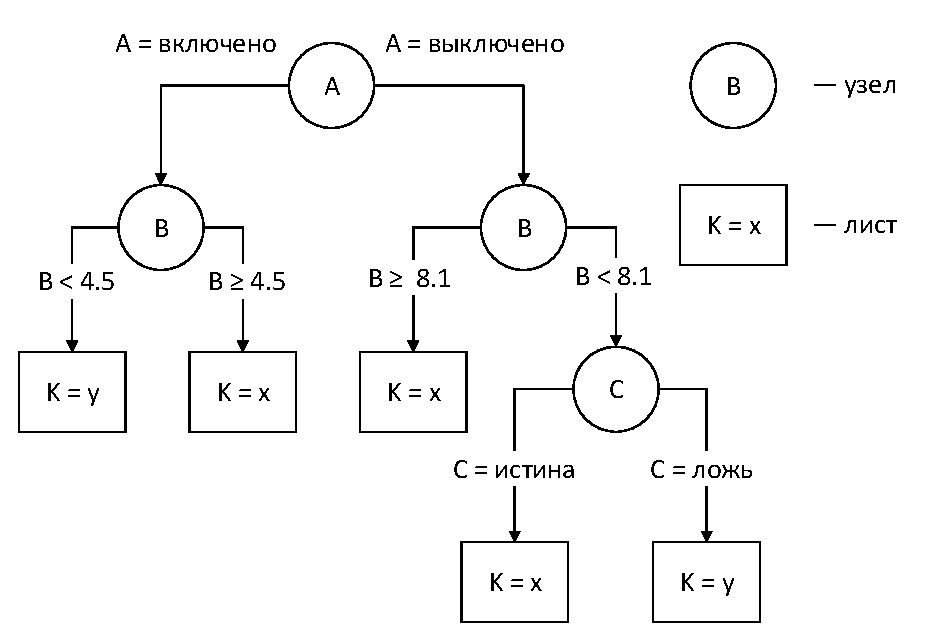
\includegraphics[width=0.7\textwidth, keepaspectratio]{decision_tree}
\caption{Пример дерева решений} \label{fig:spec:DecisionTreeExample}
\end{figure}

Так как алгоритм C4.5 относится к машинному обучению с учителем, GritBot дополняет его механизмом автоматического определения классов на основе вычисления статистических свойств выборки.

В исследовании~\cite{MLInCyberTrust} GritBot показал крайне низкую эффективность, не найдя ни одной добавленной в выборку аномалии. Это связано со статистическим подходим к определению аномальности объекта (метод ищет корреляцию между параметрами объектов в выборке). 

К преимуществам можно отнести лёгкость интерпретации результатов человеком (из-за использования деревьев решений можно получить набор правил, по которым пример был признан аномальным).

Недостатки:
\begin{itemize}
	\item низкая эффективность при наличии в выборке объектов с большим числом аномальных параметров~\cite{MLInCyberTrust};
	\item данный метод загружает весь массив исходных данных в память~\cite{BaySchwabacherOrca}; таким образом, с его помощью невозможно обрабатывать сколь-либо большие выборки;
	\item нет численной оценки степени аномальности примера (метод сортирует аномалии по их статистической значимости)~\cite{MartinCompUnsupervisedDetectionMethods}.
\end{itemize}

\subsection{GMM (Gaussian Mixture Model)}
GMM, или модель гауссовых смесей, наследует идеи Байесовской вероятности в том смысле, что она может быть легко представлена в рамках парадигмы графического моделирования.

Пример графической модели, представляющей гауссову смесь, показана на рисунке~\ref{fig:spec:GmmRepresentation}. Здесь $q_k\in \{1,\dots,M\}$, $\theta = (\pi_1,\dots,\pi_M,\mu_1,\dots,\mu_M,\Sigma_1,\dots,\Sigma_M)$. Закрашенные узлы представляют наблюдаемые непрерывные переменные, $y_k$ для момента времени $k$. Незакрашенные узлы, $q_k$, представляют $M$ ненаблюдаемых дискретных переменных, условная вероятность которых может быть вычислена на основе наблюдаемых данных. Параметры, содержащие $\theta$, могут быть выражены как функция от этих условных вероятностей и от других похоже сформированных оценок для каждой из $M$ гауссовых смесей, включая весовые коэффициенты смесей ($pi_i$), математические ожидания ($mu_i$) и матрицы ковариации ($\Sigma_i$).

\begin{figure}[h]
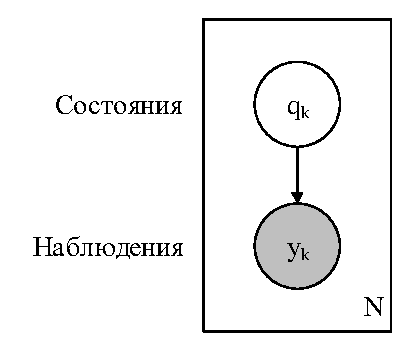
\includegraphics{gmm}
\caption{Графическое представление GMM без учителя}
\label{fig:spec:GmmRepresentation}
\end{figure}

Для использования данной модели требуется выполнение двух гипотез, представленных ниже.

\uline{Гипотеза о природе данных}: тестовые примеры появляются случайно и независимо, согласно вероятностному распределению, равному смеси распределений кластеров. Данное условие отображено в формуле~\eqref{eq:spec:GMM:Condition1}.

\begin{equation} \label{eq:spec:GMM:Condition1}
p(x) = \sum_{c\in C}^{} w_c p_c(x), \sum_{c\in C}^{} w_c = 1\text{,}
\end{equation}
\begin{description}
	\item[где $w_c$]~---~вероятность появления объектов из кластера $c$;
	\item[$p_c$]~---~плотность распределения кластера $c$.
\end{description}

\uline{Гипотеза о форме кластеров}: каждый кластер $c$ описывается $d$-мерной гауссовской плотностью с центром $\mu_c = \{\mu_{c1},\dots,\mu_{cd}\}$ и диагональной матрицей ковариации $\Sigma_c = diag(\sigma^2_{c1},\dots,\sigma^2_{cd})$ (т.е. по каждой координате своя дисперсия).

В этих предположениях для определения аномалий получается задача разделения смеси гауссовых распределений. Для этого обычно используется EM-алгоритм (expectation-maximization)~\cite{MartinCompUnsupervisedDetectionMethods}. Подробное описание данного алгоритма представлено в~\cite{KorolevEMAlgo}.

EM-алгоритм используется в математической статистике для нахождения оценок максимального правдоподобия параметров вероятностных моделей, в случае, когда модель зависит от некоторых скрытых переменных. Каждая итерация алгоритма состоит из двух шагов. На \textit{E-шаге (expectation)} вычисляется ожидаемое значение функции правдоподобия, при этом скрытые переменные рассматриваются как наблюдаемые. На \textit{M-шаге (maximization)} вычисляется оценка максимального правдоподобия, таким образом увеличивается ожидаемое правдоподобие, вычисляемое на E-шаге. Затем это значение используется для E-шага на следующей итерации. Алгоритм выполняется до сходимости.

Формальная постановка задачи разделения смеси гауссовых распределений выглядит следующим образом. Задана выбора $X^l$ случайных и независимых наблюдений из смеси $p(x)$, в которой описание $i$-го элемента есть вектор $x_i\in \mathbb{R}^n$. Принята модель, в которой каждая компонента смеси есть гауссиана с параметрами $\mu$ и $\Sigma$, и известно число компонентов смеси~---~$K$. Смесь показана в формуле~\eqref{eq:spec:GMM:Mixture}.

\begin{equation} \label{eq:spec:GMM:Mixture}
p(x) = \sum_{n=1}^{K} \pi_k N(x|\mu_k,\Sigma_k).
\end{equation}

Требуется оценить вектор параметров $\theta = (\pi_1,\dots,\pi_M,\mu_1,\dots,\mu_M,\Sigma_1,\dots,\Sigma_M)$, доставляющий максимум функции правдоподобия~\eqref{eq:spec:GMM:LikelihoodFunc}.

\begin{equation} \label{eq:spec:GMM:LikelihoodFunc}
\ln p(X|\pi,\mu,\Sigma) = \sum_{n=1}^{N} \ln \left\{\sum_{k=1}^{K} \pi_k N(x_n|\mu_k,\Sigma_k)\right\}
\end{equation}

Оптимальные параметры отыскиваются последовательно с помощью итерационного EM-алгоритма. Основная идея~–--~вводится вспомогательный вектор скрытых переменных. Это позволяет свести сложную оптимизационную задачу к последовательности итераций по пересчету коэффициентов (скрытых переменных по текущему приближению вектора параметров~---~E-шаг) и максимизации правдоподобия (с целью найти следующее приближение вектора~---~М-шаг).

В начале работы алгоритма задаются параметры начального приближения $\theta_0$. Далее итеративно выполняется следующая пара процедур:

\uline{E-шаг}: используя текущее значение вектора параметров $\theta$, вычисляется значение вектора скрытых переменных $\gamma$ по формуле~\eqref{eq:spec:GMM:HiddenVars}.

\begin{equation} \label{eq:spec:GMM:HiddenVars}
\gamma_{nk} = \frac{\pi_k N(x_n|\mu_k,\Sigma_k)}{\sum_{j=1}^{K} \pi_j N(x_n|\mu_j,\Sigma_j)}
\end{equation}

\uline{M-шаг}: переоценка вектора параметров по формулам~\eqref{eq:spec:GMM:newParams}, используя текущее значение вектора скрытых переменных.

\begin{subequations} \label{eq:spec:GMM:newParams}
\begin{equation} %\label{eq:spec:GMM:newMu}
\mu_k^{new} = \frac{1}{N_k} \sum_{n=1}^{N} \gamma_{nk} x_n \text{,}
\end{equation}
\begin{equation} %\label{eq:spec:GMM:newSigma}
\Sigma_k^{new} = \frac{1}{N_k} \sum_{n=1}^{N} \gamma_{nk} (x_n - \mu_k^{new})(x_n-\mu_k^{new})^T \text{,}
\end{equation}
\begin{equation} %\label{eq:spec:GMM:newPi}
\pi_k^{new} = \frac{N_k}{N} \text{,}
\end{equation}
\begin{equation} %\label{eq:spec:GMM:newN}
N_k = \sum_{n=1}^{N} \gamma_{nk} \text{,}
\end{equation}
\end{subequations}

Процедура останавливается после того, как норма разности векторов скрытых переменных на каждой итерации не будет превышать заданную константу~$\Delta$. Условие останова показно в~\eqref{eq:spec:GMM:StopCondition}.

\begin{equation} \label{eq:spec:GMM:StopCondition}
\delta_{max} = \max \left\{\delta_{max},|\gamma_{nk} - \gamma_{nk}^0|\right\} \leq\Delta
\end{equation}

Блок-схема алгоритма приведена в приложении~\ref{app:GMM:EMScheme}.

\subsection{Динамические байесовские сети (Dynamic Bayesian Network, DBN)}
Dynamic Bayesian Network, или динамическая байесовская сеть, является графической вероятностной моделью, представляющей собой множество переменных и их вероятностных зависимостей. Данный метод использует в своей работе формулу Байеса~\eqref{eq:spec:DBN:BayesTheorem}.

\begin{equation} \label{eq:spec:DBN:BayesTheorem}
P(A|B) = \frac{P(B|A) P(A)}{P(B)} \text{,}
\end{equation}
\begin{description}
	\item[где $P(A)$]~---~априорная вероятность гипотезы $A$;
	\item[$P(A|B)$]~---~вероятность гипотезы $A$ при наступлении события $B$ (апостериорная вероятность);
	\item[$P(B|A)$]~---~вероятность наступления события $B$ при истинности гипотезы $A$;
	\item[$P(B)$]~---~полная вероятность наступления события $B$.
\end{description}

Формула Байеса позволяет «переставить причину и следствие»: по известному факту события вычислить вероятность того, что оно было вызвано данной причиной. События, отражающие действие «причин», в данном случае называют \textit{гипотезами}, так как они~---~предполагаемые события, повлекшие данное. Безусловную вероятность справедливости гипотезы называют \textit{априорной} (насколько вероятна причина вообще), а условную~---~с учетом факта произошедшего события~---~\textit{апостериорной} (насколько вероятна причина оказалась с учетом данных о событии).

Формально байесовская сеть~---~это направленный ациклический граф, каждой вершине которого соответствует случайная переменная, а дуги графа кодируют отношения условной независимости между этими переменными. Вершины могут представлять переменные любых типов, быть взвешенными параметрами, скрытыми переменными или гипотезами. Если переменные байесовской сети являются дискретными случайными величинами, то такая сеть называется дискретной байесовской сетью. Байесовские сети, которые моделируют последовательности переменных, называют \textit{динамическими байесовскими сетями}~\cite{PearlDynamicBayesianNetworks}.

Если дуга выходит из вершины $A$ в вершину $B$, то $A$ называют родителем $B$, а $B$ называют потомком $A$. Если из вершины $A$ существует ориентированный путь в другую вершину $B$, то $B$ называется потомком $A$, а $A$ называется предком $B$. Множество вершин-родителей вершины $V_i$ обозначается как $parents(V_i) = PA_i$.

Направленный ациклический граф $G$ называется байесовской сетью для вероятностного распределения $P(v)$, заданного над множеством случайных переменных $V$, если каждой вершине графа поставлена в соответствие случайная переменная из $V$, а дуги в графе удовлетворяют условию (марковское условие): любая переменная $V_i$ из $V$ должна быть условно независима от всех вершин, не являющихся ее потомками, если заданы (получили означивание, обусловлены) все ее прямые родители $PA_i$ в графе $G$, то есть выполняется выражение~\eqref{eq:spec:DBN:BayesNetworkCondition}.

\begin{equation} \label{eq:spec:DBN:BayesNetworkCondition}
\forall V_i\in V: P(v_i|pa_i, s) = P(v_i|pa_i) \text{,}
\end{equation}
\begin{description}
	\item[где $v_i$]~---~значение $V_i$;
	\item[$S$]~---~множество всех вершин, не являющихся потомками $V_i$;
	\item[$s$]~---~конфигурация $S$;
	\item[$pa_i$]~---~конфигурация $PA_i$.
\end{description}

Тогда полное совместное распределение значений в вершинах можно удобно записать в виде декомпозиции (произведения) локальных распределений~\eqref{eq:spec:DBN:Distributions}.

\begin{equation} \label{eq:spec:DBN:Distributions}
P(V_1,\dots,V_n) = \prod_{i=1}^{n} P(V_i|parents(V_i))
\end{equation}

Если у вершины $V_i$ нет предков, то её локальное распределение вероятностей называют \textit{безусловным}, иначе \textit{условным}. Если вершина~---~случайная переменная получила означивание (например, в результате наблюдения), то такое означивание называют \textit{свидетельством}. Если значение переменной было установлено извне (а не наблюдалось), то такое означивание называется \textit{вмешательством} или \textit{интервенцией}~\cite{PearlDynamicBayesianNetworks}.

Условная независимость в байесовской сети представлена графическом свойством \textit{d-разделённости}. Пусть $X, Y, Z$~---~непересекающиеся подмножества вершин в ацикличном ориентированном графе $G$. Говорят, что множество вершин $Z$ d-разделяет $X$ и $Y$ тогда и только тогда, когда $Z$ блокирует все пути из любой вершины, принадлежащей $X$, в любую вершину, принадлежащую $Y$. Под путём понимается последовательность следующих друг за другом рёбер (любого направления) в графе.

В соответствии с теоремой о d-разделённости для ациклично ориентированного графа $G$ если вершины d-разделены, то они условно независимы; и если вершины условно-независимы во всех вероятностных распределениях, совместимых с графом G, то они d-разделены~\cite{PearlDynamicBayesianNetworks}.

Для динамических байесовских сетей существуют две возможных стратегии для поиска аномалий~\cite{DBNAnomalyDetection}: байесовский доверительный интервал (Bayesian Credible Interval, BCI) и максимальная апостериорная оценка измерений (maximum a posteriori measurement status, MAP-ms).

\subsubsection{Байесовский доверительный интервал (BCI)}
\label{subsubsec:spec:DBN:BCI}
Данная стратегия использует модель сети, представленную на рисунке~\ref{fig:spec:DBN:BCI}. Вектор $X$ представляет скрытые непрерывные переменные, вектор $M$~---~наблюдаемые непрерывные переменные. Нижние индексы обозначают моменты времени.

\begin{figure}[h]
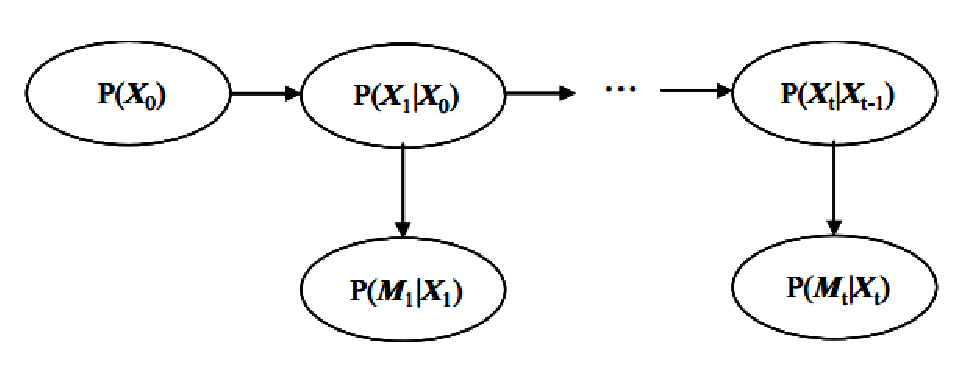
\includegraphics[width=0.7\textwidth]{dbn_bci}
\caption{Графическая модель сети для байесовского интервала правдоподобия (BCI)}
\label{fig:spec:DBN:BCI}
\end{figure}

Такая байесовская сеть отслеживает многомерные распределения линейных гауссовых переменных состояния и их наблюдаемые аналоги, которые измеряются с помощью датчиков. Скрытые переменные полагаются Марковскими процессами первого порядка, т.е. значение переменной в момент времени $t$ зависит только от состояния в момент времени $t-1$. Апостериорные вероятности скрытых и наблюдаемых переменных получаются с помощью фильтра Калмана, как только поступают новые измерения с датчиков. Данные вероятности используются для построения байесовского доверительного интервала $p\%$. Апостериорная вероятность $p$ отражает тот факт, что наблюдаемая переменная находится внутри интервала. Таким образом, любое измерение, попадающее за пределы доверительного интервала $p\%$, может быть классифицировано как аномалия~\cite{DBNAnomalyDetection}. Параметры сети (распределения вероятностей $P(X_0), P(X_t|X_{t-1}), P(M_t|X_t)$) могут быть получены из исходной выборки с помощью EM-алгоритма~\cite{KorolevEMAlgo}.

\subsubsection{Максимальная апостериорная оценка измерений (MAP-ms)}
В стратегии MAP-ms используется более сложная модель сети, показанная на рисунке~\ref{fig:spec:DBN:MAPms}. Векторы $X$ и $Z$ представляют непрерывные и дискретные скрытые переменные, а вектор $M$~---~наблюдаемые непрерывные переменные. Нижние индексы обозначают моменты времени.

\begin{figure}[h]
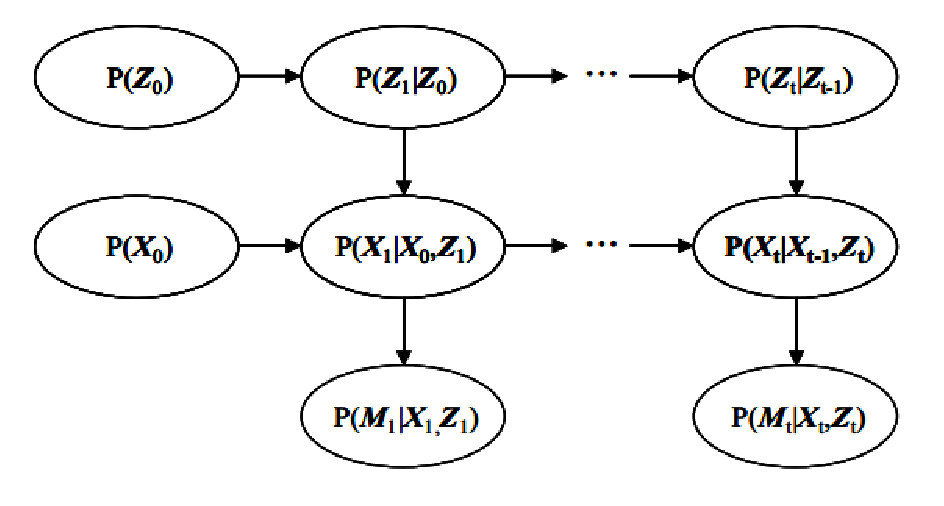
\includegraphics[width=0.7\textwidth]{dbn_mapms}
\caption{Графическая модель сети для максимального апостериорного статуса измерений (MAP-ms)}
\label{fig:spec:DBN:MAPms}
\end{figure}

Данная модель отслеживает многомерные многомерные распределения линейных гауссовых переменных состояния и их наблюдаемые аналоги, которые измеряются с помощью датчиков, как и вероятности скрытых дискретных переменных, показывающих статус каждого измерения (например, номинальный/аномальный). К примеру, если есть две измеряемых переменных состояния, то дискретная переменная статуса измерения будет иметь четыре возможных значения: (номинальный, номинальный), (аномальный, номинальный), (номинальный, аномальный) и (аномальный, аномальный). Апостериорные вероятности скрытых и наблюдаемых переменных получаются с помощью фильтра частиц Рао-Блэквелла, как только поступают новые измерения с датчиков. Максимальная апостериорная оценка измерения (например, наиболее вероятное значение, полученное из апостериорной вероятности) скрытой переменной состояния, показывающей статус измерения, может быть использована для классификации измерения как номинального или аномального. 

MAP-ms для работы требует, во-первых, параметры байесовской сети, описывающие изменение во времени линейных гауссовых переменных состояния для каждого значения дискретного статуса измерения, и, во-вторых, параметры, описывающие изменение во времени дискретных переменных. Кроме того, необходимо вручную задать вероятности для дискретных переменных ($P(Z_0), P(Z_t|Z_{t-1})$), опираясь на знание предметной области. Для случая, когда аномалий в исходной выборке нет, параметры сети совпадают с сетью для стратегии BCI, описанной в пункте~\ref{subsubsec:spec:DBN:BCI}. Если же одно или несколько измерений являются аномальными, параметры сети могут довольно сильно отличаться.~\cite{DBNAnomalyDetection}

Основные преимущества динамических байесовских сетей в применении к обнаружению аномалий:
\begin{itemize}
	\item способность работать в режиме реального времени~\cite{DBNAnomalyDetection};
	\item возможнсть графически представить модель системы.
\end{itemize}

Недостатки:
\begin{itemize}
	\item крайне высокая сложность метода;
	\item низкая эффективность на реальных данных~\cite{MartinCompUnsupervisedDetectionMethods}.
\end{itemize}